%+++++++++++++++++++++++++++++++++++++++++++++++++++++++++++++++
% SUMMARY    : Lecture 14
%            : University of Southern Maine 
%            : @james.quinlan
%            : John Parks
%+++++++++++++++++++++++++++++++++++++++++++++++++++++++++++++++



\section*{Objectives}
\begin{outline}
    \1 Optimizers
    \1 Gradient Descent
\end{outline}

\rule[0.0051in]{\textwidth}{0.00025in}
% ----------------------------------------------------------------

\section*{Optimizers}

\underline{Goal: } Find "test" value: maximize or minimize

\underline{Loss function: } minimize
Two methods
\begin{itemize}
    \item exact take derivative = 0
    \item  Gradient-based method
\end{itemize}



\tikzset{every picture/.style={line width=0.75pt}} %set default line width to 0.75pt        

\begin{tikzpicture}[x=0.75pt,y=0.75pt,yscale=-1,xscale=1]
%uncomment if require: \path (0,310); %set diagram left start at 0, and has height of 310

%Curve Lines [id:da4742299429119865] 
\draw    (100,118) .. controls (140,88) and (116.86,244.29) .. (170.86,148.29) ;
%Curve Lines [id:da9458592077548552] 
\draw    (170.86,148.29) .. controls (199.86,97.29) and (155.86,234.29) .. (208.86,160.29) ;
%Curve Lines [id:da2473829104686256] 
\draw    (208.86,160.29) .. controls (248.86,130.29) and (213.86,316.29) .. (301.86,114.29) ;

%Flowchart: Connector [id:dp7205102074241437] 
\draw   (139,177.6) .. controls (139,175.06) and (141.06,173) .. (143.6,173) .. controls (146.14,173) and (148.2,175.06) .. (148.2,177.6) .. controls (148.2,180.14) and (146.14,182.2) .. (143.6,182.2) .. controls (141.06,182.2) and (139,180.14) .. (139,177.6) -- cycle ;
%Flowchart: Connector [id:dp8727380534288091] 
\draw   (176,135.6) .. controls (176,133.06) and (178.06,131) .. (180.6,131) .. controls (183.14,131) and (185.2,133.06) .. (185.2,135.6) .. controls (185.2,138.14) and (183.14,140.2) .. (180.6,140.2) .. controls (178.06,140.2) and (176,138.14) .. (176,135.6) -- cycle ;
%Flowchart: Connector [id:dp9540866612980529] 
\draw   (181,181.6) .. controls (181,179.06) and (183.06,177) .. (185.6,177) .. controls (188.14,177) and (190.2,179.06) .. (190.2,181.6) .. controls (190.2,184.14) and (188.14,186.2) .. (185.6,186.2) .. controls (183.06,186.2) and (181,184.14) .. (181,181.6) -- cycle ;
%Flowchart: Connector [id:dp4621401791397879] 
\draw   (214,156.6) .. controls (214,154.06) and (216.06,152) .. (218.6,152) .. controls (221.14,152) and (223.2,154.06) .. (223.2,156.6) .. controls (223.2,159.14) and (221.14,161.2) .. (218.6,161.2) .. controls (216.06,161.2) and (214,159.14) .. (214,156.6) -- cycle ;
%Flowchart: Connector [id:dp5695502833856403] 
\draw   (241,209.6) .. controls (241,207.06) and (243.06,205) .. (245.6,205) .. controls (248.14,205) and (250.2,207.06) .. (250.2,209.6) .. controls (250.2,212.14) and (248.14,214.2) .. (245.6,214.2) .. controls (243.06,214.2) and (241,212.14) .. (241,209.6) -- cycle ;
%Flowchart: Connector [id:dp9531625467829591] 
\draw  [fill={rgb, 255:red, 0; green, 0; blue, 0 }  ,fill opacity=1 ] (106,116.6) .. controls (106,114.06) and (108.06,112) .. (110.6,112) .. controls (113.14,112) and (115.2,114.06) .. (115.2,116.6) .. controls (115.2,119.14) and (113.14,121.2) .. (110.6,121.2) .. controls (108.06,121.2) and (106,119.14) .. (106,116.6) -- cycle ;




\end{tikzpicture}

Initial value = seed the generator

\section{Vanilla Gradient Descent}

\underline{Update function:} \boxed{w_{t+1}=w_{t}-\gamma \nabla L(w_t)} \\
L(W) is the loss function\\
$\gamma$ is the learning rate, a hyperparameter tunable via cross-validation\\ 





\tikzset{every picture/.style={line width=0.75pt}} %set default line width to 0.75pt        

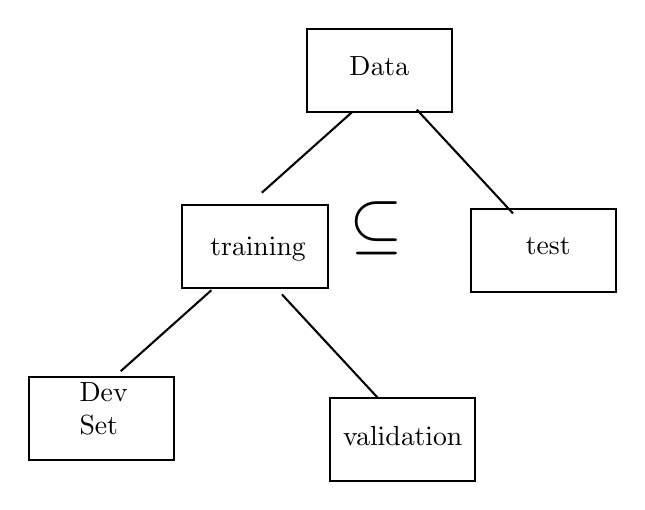
\begin{tikzpicture}[x=0.75pt,y=0.75pt,yscale=-1,xscale=1]
%uncomment if require: \path (0,310); %set diagram left start at 0, and has height of 310

%Shape: Rectangle [id:dp043925721141883645] 
\draw   (153,41) -- (223,41) -- (223,81) -- (153,81) -- cycle ;
%Shape: Rectangle [id:dp7328778113397988] 
\draw   (232,128) -- (302,128) -- (302,168) -- (232,168) -- cycle ;
%Shape: Rectangle [id:dp2799764635525812] 
\draw   (93,126) -- (163,126) -- (163,166) -- (93,166) -- cycle ;
%Shape: Rectangle [id:dp7386837970903096] 
\draw   (19,209) -- (89,209) -- (89,249) -- (19,249) -- cycle ;
%Shape: Rectangle [id:dp30144424145198556] 
\draw   (164,219) -- (234,219) -- (234,259) -- (164,259) -- cycle ;
%Straight Lines [id:da2550368319027301] 
\draw    (206,80) -- (252.33,130) ;
%Straight Lines [id:da7481890861248687] 
\draw    (141,169) -- (187.33,219) ;
%Straight Lines [id:da9401859557306093] 
\draw    (175,81) -- (131.33,120) ;
%Straight Lines [id:da40684207122585114] 
\draw    (107,167) -- (63.33,206) ;

% Text Node
\draw (172,53) node [anchor=north west][inner sep=0.75pt]   [align=left] {Data};
% Text Node
\draw (257,140) node [anchor=north west][inner sep=0.75pt]   [align=left] {test};
% Text Node
\draw (105,140) node [anchor=north west][inner sep=0.75pt]   [align=left] {training};
% Text Node
\draw (42,210) node [anchor=north west][inner sep=0.75pt]   [align=left] {Dev\\Set};
% Text Node
\draw (169,231) node [anchor=north west][inner sep=0.75pt]   [align=left] {validation};
% Text Node
\draw (172,123) node [anchor=north west][inner sep=0.75pt]  [font=\Huge] [align=left] {$\displaystyle \subseteq $};


\end{tikzpicture}
\\
frequent issues:\\
\begin{itemize}
    \item gets stuck at local minimum 
    \item vanishing gradient
    \item If the learning rate is increased, it can get unstuck but risks jumping over desired points if increased too much
    
\end{itemize}


\section{Momentum}
\underline{Intuitive: } $w_{t+1}=w_t-\gamma \nabla L(w_t) + \text{(past gradients)}$\\
\underline{Actual: }\boxed{v_0=0}\\ \boxed{v_{t+1}=\xi v_t + \nabla L(w_t)}
\boxed{w_{t+1}=w_t-\gamma v_{t+1}}\\
\underline{issue: } can move past desired point because of momentum of past gradients\\
\underline{evaluating performance: } \fbox{Count number of iterations}\\

\section{Gradient-Based Nesterov}
\boxed{v_0=0}\\
\boxed{v_{t+1}=\xi v_t + \nabla L(w_t)}
\boxed{w_{t+1}=w_t-\gamma (\delta v_{t+1} + \nabla L(w_t))}\\
look ahead : $\delta v_{t+1}$

